%$Id$
\documentclass[conference, compsoc]{IEEEtran}
\usepackage{fontspec}
%\usepackage{amsmath,amssymb,amsthm,supertabular,booktabs,rotating,semantic,subfigure,multirow,colortbl}
\usepackage{graphicx, url, subfigure}
\usepackage[colorlinks=true,linkcolor=black,anchorcolor=black,citecolor=black,urlcolor=black,bookmarks=false,pdfstartview=FitH]{hyperref}
\usepackage{algorithmic,algorithm}
\usepackage{xunicode}
\usepackage{colortbl,longtable}
\usepackage{xltxtra}
\defaultfontfeatures{Mapping=tex-text}
\setmainfont{Times New Roman}
\begin{document}

\bibliographystyle{IEEEtran}
 
\title{Understanding software quality evolution using signifier frequency extraction}
\author{
Neil A. Ernst\\Dept. of Computer Science\\University of Toronto\\nernst@cs.toronto.edu \and
John Mylopoulos\\Dept. of Computer Science\\University of Toronto\\jm@cs.toronto.edu }

\maketitle

\begin{abstract}
This paper describes a software repository mining technique we call signifier extraction. Signifiers are keywords about software quality that we generate using Wordnet and the ISO quality taxonomy. Using corpora created from eight Gnome projects -- their mailing lists, subversion comments, and bug comments -- we search for the signifiers over three month, quarterly intervals. The occurrence of our signifiers forms an evolutionary pattern that we analyze statistically and historically. We show that it is possible to reconstruct the historical evolution of software qualities as responses to external forcings, such as release cycles and usability audits. %[numbers?]
\end{abstract}

\section{Introduction}\label{sect:introduction}%Aim
\begin{quote}[My impression] is of a large project in a state of marginal returns, in which a larger and larger part of the effort goes to maintenance. -- Andy Wingo, Gnome developer, June 2008.\footnote{http://wingolog.org/archives/2008/06/07/gnome-in-the-age-of-decadence}\end{quote}
	This quote, from a developer in the Gnome ecosystem, captures some of what this paper tries to explain. Is it the case that as projects mature the focus and effort of the developers must turn to maintenance tasks\cite{Swanson1976}? Certainly Lehman's conclusion~\cite{lehman_software_2006} is that this is the case (viz. Lehman's 7th `law'). This paper takes up the question as to whether this can be empirically demonstrated. To test this notion, we begin with a few assumptions. The first is that there is some sort of signal we can capture that will signify that `maintenance' is being done. One approach is to scan code for maintenance activity, using, for example, formal concept analysis~\cite{breu06msr}. Our approach, by contrast, is focused on the conversations developers have (with each other, or with `users'). To identify when `effort goes to maintenance', we begin by assuming that discussions about maintenance often involve a set of common terms, which we call signifiers. We define these using the ISO 9126-1 software quality model \cite{iso9126} as a starting point. 

[some mention of how this is an exploratory study]	
	
Section \ref{sec:Method} describes how we derive these signifiers and how we built our corpora and toolset for extracting the signifiers. We then present our observations and a discussion about significance in Section \ref{sec:observations}. Finally, we examine some threats to our approach and discuss related work. 

\begin{figure}[b]
\centering
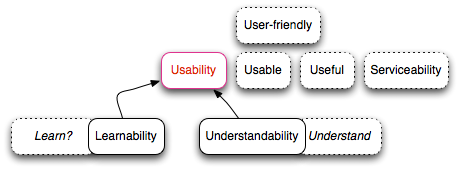
\includegraphics[width=0.4\textwidth]{synonym-graph.pdf}
\caption{An extensional definition of usability, showing in dashed lines those concepts outside our signifier `bubble'.}
\label{fig:syngraph}
\end{figure}
	
\section{Methodology}
\label{sec:Method}
Our dataset is a selection of eight Gnome projects (listed on the Gnome wiki), shown in Table \ref{tbl:projects}. The projects were selected to represent a variety of lifespans (from 18 months to 11 years) and code sizes. For each project we extracted text-based datasets: that project's mailing list (except for Ekiga and Empathy which have no apparent mailing list); that project's subversion logs; and finally, the bug comments for the project. We extracted the date, text (which we term an `event'), and source, and placed this information into a MySQL database.

\subsection{Signifier extraction}
\begin{table}
	\caption{Selected Gnome ecosystem products}
	\centering
	\label{tbl:projects}
\begin{tabular}{|c|c|c|c|}
\hline
\rowcolor[gray]{.9} 
\textbf{Product} & \textbf{Language} & \textbf{Size} \emph{(Kloc)} & \textbf{Age} \emph{(years)} \\
\hline
\hline 
Evolution & C & 313 & 10.75\\ \hline
Nautilus & C & 108 & 10.75  \\ \hline
Metacity & C & 66 & 7.5  \\ \hline
Ekiga & C++ & 54 & 7  \\ \hline
Totem & C & 49 & 6.33  \\ \hline
Deskbar & Python/Sh & 21 & 3.2  \\ \hline
Evince & C & 66 & 9.75\\ \hline
Empathy &C & 55 & 1.5\\ 
\hline
\end{tabular}
\end{table}

In semiotics, Peirce drew a distinction drawn between signifier, signified, and sign~\cite{atkin2006}. In this work, we make use of signifiers -- words like `usability' and `usable' -- to capture the occurrence in our corpora of the signified -- in this example, the concept `usability'. We extract our signified, concept words from the ISO 9126 quality model~\cite{iso9126}. There is some debate about the significance and importance of the terms in this model. However, it is ``an international standard and thus provides an internationally accepted terminology for software quality~\cite[p. 58]{Boegh2008},'' which is sufficient for the purposes of this research. The model is used to refer to both external and internal views of quality (for example, bugs filed by users would be external qualities, whereas an email discussion of features to come would be internal). We generate the signifiers from Wordnet~\cite{Fellbaum1998}, an English-language `lexical database' that contains semantic relations between words, including meronymy and synonymy. We extract words using the procedure defined in \ref{alg1}. The only deviation we made was to add the term `performance' to the synonyms for `efficiency', since this seems like a common synonym in this domain (Wordnet is not domain-specific). %This factor shows up in the higher error rates, particulary for two word terms like time behaviour.

\renewcommand{\algorithmiccomment}[1]{// #1}
\begin{algorithm}[H]
\caption{Defining signified terms extensionally}
  \label{alg1}
\begin{algorithmic}
	\REQUIRE $T$, the set of top-level terms in ISO9126-1
  	\FORALL{$t \in T$}
	\STATE $S \leftarrow \emptyset $
    %\STATE define $t$ as a wordnet noun
	\STATE identify synset of $t$ (synonyms)%  from Wordnet
	\STATE $S \leftarrow S +$ synset
	\STATE identify direct hypernyms of $t$ (specializations)% from Wordnet
	\STATE $S \leftarrow S +$ hypernyms %is-a
	\STATE identify meronyms of $t$ (components)% from ISO9126
	\STATE $S \leftarrow S +$ meronyms %part-of
	\STATE identify related forms of $t$ (stemmed)% from Wordnet
	\STATE $S \leftarrow S +$ related forms
	\FORALL {$s \in S$}
		\STATE query corpora for $s$
		\COMMENT ignore case
	\ENDFOR
  \ENDFOR
\RETURN $E$, the set of unique `events' per $t$

\end{algorithmic}
\end{algorithm}
Note, we do not currently look for common misspellings or other languages (the primary language is English, at any rate). This algorithm gives us a linguistic `bubble' which we use to extensionally define the signified term, as shown in Fig. \ref{fig:syngraph}. An event is any row in the table which contains at least one term in the bubble (i.e., don't double count). 

Our MySQL queries produced a set of unique events (e.g., a subversion commit message), averaged over quarters of years, and the associated time and project. From this we conducted our observations and statistical tests.

\section{Observations}
\label{sec:observations}
Fig. \ref{fig:ev-func-line} and Fig. \ref{fig:ev-eff-line} show two examples of our queries. The red line connects a number of events for that particular quarter. For example, in the third quarter of 2000, there were approximately 80 normalized events in the Evolution project for Efficiency. We normalize the extracted event numbers to remove the effect of mailing list volume changes or commit log volumes. The calculation takes the extracted events, divides by the total events, and multiplies by 1000. The black line is a first-order regression line, and the dashed vertical lines represent Gnome project milestones, with which most of the projects we study are synchronized.
 
% \begin{figure*}[h]
% \centering
% 	\subfigure[][]{
% 		{\includegraphics[width=0.7\textwidth]{figures/Evolution-Functionalityline.png}}
% 	}%{Evolution product, Functionality quality. Trend is positive, with some clear spikes before major releases.}
% 	\subfigure[][]{
% 		{\includegraphics[width=0.4\textwidth]{figures/Evolution-Efficiencyline.png}}
% 	}%{Evolution product, Efficiency quality. Trend is negative, with some clear spikes after major releases.}
% \label{fig:ev-line}
% \caption{dull}
% \end{figure*}

\begin{figure}[h]
	\centering
	\includegraphics[width=0.5\textwidth]{figures/Evolution-Efficiencyline.png}
\label{fig:ev-eff-line}
\caption{Evolution product, Efficiency quality. Trend is negative, with some clear spikes after major releases.}
\end{figure}

\begin{figure}[h]
\centering
\includegraphics[width=0.5\textwidth]{figures/Evolution-Functionalityline.png}
\label{fig:ev-func-line}
\caption{Evolution product, Functionality quality. Trend is positive, with some clear spikes before major releases.}
\end{figure}

%[Compare excerpt text to events, eg the usability event in Evolution]
%[where the quarter is ended is important...]
\subsection{Discussion}
We include a linear regression of the number of occurrences against the date. The equation of the regression line shows the average value of the number of occurrences as the date increases. A linear relationship may not be a good model of the actual pattern. For example, the number of occurrences may be changing in response to some other variable, such as co-ordinated release dates (plotted as vertical gray lines, above); developer illness, and many others. In many ways this is the purpose of this set of experiments. Nonetheless, one of the key questions this research project initially proposed was `does quality become of greater interest as a project matures', which is shown by the linear regression line. To measure the significance of this relationship, we also measure the squared correlation value, $r^2$, in percentage, where 100\% indicated perfect correlation.
%Multi-level modeling

\begin{table}
	\caption{Selected summary statistics}
	\centering
	\label{tbl:projects}
\begin{tabular}{|c|c|c|}
\hline
\rowcolor[gray]{.9} 
File-Keyword &  $r^2$ &  slope \\
Evolution-Efficiency & 0.07 & -0.38 \\
Evolution-Portability & 0.12 & -0.36 \\
Evolution-Maintainability & 0.05 & -0.27 \\
Evolution-Reliability & 0.08 & -0.29 \\
Evolution-Functionality & 0.05 & 0.92 \\
Evolution-Usability & 0.12 & -1.38 \\
Nautilus-Efficiency & 0.19 & -4.77 \\
Nautilus-Portability & 0.11 & -0.51 \\
Nautilus-Maintainability & 0.37 & -1.49 \\
Nautilus-Reliability & 0.38 & -1.00 \\
Nautilus-Functionality & 0.26 & -4.22 \\
Nautilus-Usability & 0.23 & -7.96 \\
Totem-Efficiency & 0.03 & -1.86 \\
Totem-Portability & 0.06 & -0.35 \\
Totem-Maintainability & 0.00 & 0.02 \\
Totem-Reliability & 0.02 & 0.19 \\
Totem-Functionality & 0.16 & -1.87 \\
Totem-Usability & 0.33 & -1.97 \\
\hline
\end{tabular}
\end{table}

\paragraph{Explanatory theories}
One possible explanation for the behaviour of our datasets, which are only loosely correlated with time, is that events are dictated by a change in release cycle. For example, the conjecture is that as a major Gnome release gets closer, more discussion occurs of efficiency, for example. \\
\emph{Set windows at each release to see what is happening prior and after the release (e.g., unit of analysis becomes the release period, not `quarters')\\
}
The second explanation is that the data are independent of software age, or release cycle, and are instead responding to external events. For example, there may be a usability audit, or a review by a major news source of the performance of the project, etc. \\
\emph{Analysis of key peaks in selected graphs}
\subsection{Error checking}
We performed some (simple) error checking on our results. What we wanted to verify was the percentage of terms retrieved that were unrelated to a software quality. For example, we encountered some mail messages from individuals whose email signature included the words ``Usability Engineer''. If the body of the message wasn't obviously about usability, we coded this as a false-positive. We did not assess the rate of false-negatives (as mentioned above). Our tests involved randomly selecting messages from the corpora and coding them as relevant or irrelevant. We assessed 100 events per signified term to generate our rates. Table \ref{tbl:error} presents the results of this test. In general, false-positives averaged less than 10\% of the events.

\begin{table}
	\caption{False positive rates}
	\centering
	\label{tbl:error}
\begin{tabular}{|c|c|}
\hline
Signified quality & F.P. Rate  \\
\hline
\hline
Usability & 0.06\\ \hline
Portability & \\ \hline
Maintainability & \\ \hline
Reliability & \\ \hline
Functionality & \\ \hline
\hline
\end{tabular}
\end{table}

\subsection{Threats to validity}
missing words and phrases that are related to the signifier but don't contain it (e.g., ``can't find the submit button" vs. ``usability")). \\
normalize? We don't, because we are interested in absolute numbers. For example, suppose that in the month prior to the release we get a huge spike in mailing list traffic, as the developers work out the features to be frozen. We want to retain the absolute number of events, not relative. Maybe not, maybe we want both.\\
Some words are not well-defined in general purpose ways like Wordnet or general dictionaries.\\
Some signified terms are defined by more signifiers, which should skew their occurrence counts.\\
\subsection{Related Work}
Part of our efforts with this project is to reconstruct a history of the software product's evolution, a notion we first discussed in \cite{Ernst07icsm}. That idea is derived from, in part, work on narratives of software systems shown in academic work like \cite{Anton2001} or more general-purpose works like \cite{waldo93}. Software mining of the type we do, a type of reverse formal concept analysis, is less common. Similarities exist with approaches that begin with structured taxonomies, as with the Hismo software ontology \cite{Girba2006}. Hindle et al., in \cite{hindle09icpc}, use machine learning to classify code commits into maintenance categories. It would be interesting to extend this system with pre-determined concepts.

\section{Future work and conclusions}
[did we see a trend]

[social element: who is doing what, new people come in case study?] ~\cite{Scacchi2002} on requirements for developing OSS software.

[other sources, eg Gnome usability mailing list] %http://mail.gnome.org/mailman/listinfo/usability]
\section{Appendix}
Source code, processed data, and related discussions are available at \url{http://neilernst.net/archives/tag/msr/}.
\begin{footnotesize}
\bibliography{msr}
\end{footnotesize}
\end{document}



% I suspect the underlying problem you are having is how
% to cope with requirements churn. From Mary Poppendieck's
% book "Implementing Lean Software Development" there's this
% very valuable tip:
% 
% "If you have requirements churn, you are specifying too
% early".